% !TeX spellcheck = <none>
\documentclass[11pt]{charter}

% El títulos de la memoria, se usa en la carátula y se puede usar el cualquier lugar del documento con el comando \ttitle
\titulo{Sistema de monitoreo de redes de distribución de baja tensión utilizando sensores autónomos y LoRaWAN} 

% Nombre del posgrado, se usa en la carátula y se puede usar el cualquier lugar del documento con el comando \degreename
\posgrado{Carrera de Especialización en Sistemas Embebidos} 
%\posgrado{Carrera de Especialización en Internet de las Cosas} 
%\posgrado{Carrera de Especialización en Intelegencia Artificial}
%\posgrado{Maestría en Sistemas Embebidos} 
%\posgrado{Maestría en Internet de las cosas}

% Tu nombre, se puede usar el cualquier lugar del documento con el comando \authorname
\autor{Milton Eduardo Sosa} 

% El nombre del director y co-director, se puede usar el cualquier lugar del documento con el comando \supname y \cosupname y \pertesupname y \pertecosupname
\director{Ing. Marcelo E. Romeo}
\pertenenciaDirector{Universidad Nacional de San Martín} 
% FIXME:NO IMPLEMENTADO EL CODIRECTOR ni su pertenencia
\codirector{} % si queda vacio no se deberíá incluir 
\pertenenciaCoDirector{}

% Nombre del cliente, quien va a aprobar los resultados del proyecto, se puede usar con el comando \clientename y \empclientename
\cliente{Ing. Milton Eduardo Sosa}
\empresaCliente{}

% Nombre y pertenencia de los jurados, se pueden usar el cualquier lugar del documento con el comando \jurunoname, \jurdosname y \jurtresname y \perteunoname, \pertedosname y \pertetresname.
\juradoUno{Nombre y Apellido (1)}
\pertenenciaJurUno{pertenencia (1)} 
\juradoDos{Nombre y Apellido (2)}
\pertenenciaJurDos{pertenencia (2)}
\juradoTres{Nombre y Apellido (3)}
\pertenenciaJurTres{pertenencia (3)}
 
\fechaINICIO{27 de junio de 2020}		%Fecha de inicio de la cursada de GdP \fechaInicioName
\fechaFINALPlanificacion{22 de Julio de 2021} 	%Fecha de final de cursada de GdP
\fechaFINALTrabajo{30 de Julio de 2020}		%Fecha de defensa pública del trabajo final


\begin{document}

\maketitle
\thispagestyle{empty}
\pagebreak


\thispagestyle{empty}
{\setlength{\parskip}{0pt}
\tableofcontents{}
}
\pagebreak


\section{Registros de cambios}
\label{sec:registro}


\begin{table}[ht]
\label{tab:registro}
\centering

\begin{tabularx}{\linewidth}{@{}|c|X|c|@{}}
\hline
\rowcolor[HTML]{C0C0C0} 
Revisión & \multicolumn{1}{c|}{\cellcolor[HTML]{C0C0C0}Detalles de los cambios realizados} & Fecha      \\ \hline
1.0      & Creación del documento                                                          & 22/06/2020 \\ \hline
1.1      & Avances hasta el desglose de trabajo en tareas.                                                                         																						   & 10/07/2020 \\ \hline

\end{tabularx}
\end{table}

\pagebreak



\section{Acta de Constitución del Proyecto}
\label{sec:acta}

\begin{flushright}
Buenos Aires, \fechaInicioName
\end{flushright}

\vspace{2cm}

Por medio de la presente se acuerda con el Ing. \authorname\hspace{1px} que su Trabajo Final de la \degreename\hspace{1px} se titulará ``\ttitle'', consistirá esencialmente en el prototipo preliminar de un sistema embebido de tipo autónomo que sea capaz de manera no invasiva de determinar valores eficaces de corriente alterna en sistemas metropolitanos de distribución de energía eléctrica en baja tensión y reportar estados a un centro de operaciones a través de una red LoRaWAN. Tendrá un presupuesto preliminar estimado de 600 hs de trabajo y \$60.000, sesenta mil pesos argentinos, con fecha de inicio \fechaInicioName\hspace{1px} y fecha de presentación pública \fechaFinalName.

Se adjunta a esta acta la planificación inicial.

\vfill

% Esta parte se construye sola con la información que hayan cargado en el preámbulo del documento y no debe modificarla
\begin{table}[ht]
\centering
\begin{tabular}{ccc}
\begin{tabular}[c]{@{}c@{}}Ariel Lutenberg \\ Director posgrado FIUBA\end{tabular} &  & \begin{tabular}[c]{@{}c@{}}\clientename \\ \empclientename \end{tabular} \vspace{2.5cm} \\ 
\multicolumn{3}{c}{\begin{tabular}[c]{@{}c@{}} \supname \\ Director del Trabajo Final\end{tabular}} \vspace{2.5cm} \\
\begin{tabular}[c]{@{}c@{}}\jurunoname \\ Jurado del Trabajo Final\end{tabular}     &  & \begin{tabular}[c]{@{}c@{}}\jurdosname\\ Jurado del Trabajo Final\end{tabular}  \vspace{2.5cm}  \\
\multicolumn{3}{c}{\begin{tabular}[c]{@{}c@{}} \jurtresname\\ Jurado del Trabajo Final\end{tabular}} \vspace{.5cm}                                                                     
\end{tabular}
\end{table}




\section{Descripción técnica-conceptual del Proyecto}
\label{sec:descripcion}

\begin{consigna}{black}
El presente trabajo surge como idea del autor en base a la necesidad de permitir a las redes distribución metropolitanas y megalopolitanas de integrar características de Ciudades Inteligentes y así permitir enmarcarlas dentro del concepto de Internet de las cosas (IoT). El mismo sigue las premisas de minimizar impactos y costos de implementación en las redes de distribución actual y a la vez procura lograr un aumento en la calidad de servicio de distribución de energía eléctrica haciendo uso de los datos relevados.\\
Es menester mencionar que este trabajo es parte de un proyecto de PyME de base tecnológica con el objeto de comercializar servicios a diferentes prestadoras del servicio de distribución de energía electrica en Sudamérica, como así también a personas que deseen monitorear el estado de una carga eléctrica en particular haciendo uso de una estructura de red de comunicación de largo alcance.\\
Dado el costo monetario y operativo que actualmente representa reemplazar actores clave en un sistema de distribución de energía eléctrica, como son los transformadores de media a baja tensión o bien los fusibles aéreos inmediatamente a la salida de los transformadores ya operativos en una red de distribución de energía eléctrica sin otra prestación técnica mas que bajar el nivel de tensión o proteger las líneas de una sobrecarga de corriente, surge la necesidad de proponer alternativas tecnologicas para aumentar la calidad del servicio de distribución de energía eléctrica.\\
El siguiente sistema ocuparía un mínimo espacio físico adicional en la red, pero de gran relevancia para realizar un relevamiento en tiempo semi real del estado de operación de la red de distribución de energía eléctrica.\\
Entre las características técnicas que sobresalen de este sistema, se encuentran la utilización tecnologías de redes de comunicación públicas de largo alcance y bajo consumo para reportar el estado de operación de un nodo en particular de la red. Tambien propone el uso de formas de conversión y acumulación de energía eléctrica de bajo impacto medioambiental con el objeto de lograr autonomía de operación aún en condiciones meteorológicas desfavorables y operando en régimen 24/7. Finalmente es la intención de que este prototipo se mantenga agnóstico a la frecuencia de operación de la red como así tambien a la tensión otorgando así, facilidad a la hora de realizar el comisionamiento en diferentes redes.\\


\section{Diagrama de bloques del proyecto}
El sistema propuesto se compondrá por un Hardware (HW) a desarrollar para cada nodo y los servicios interconectados en la nube también llamados Backend services (BES).\\
\subsection{Hardware a desarrollar}
\label{sec:diagrama_de_bloques_HW}

El diagrama de bloques del HW a desarrollar es presentado en la Figura \ref{fig:diagBloques}. Este posee cinco etapas:
\vspace{25px}

\begin{figure}[H]
	\centering 
	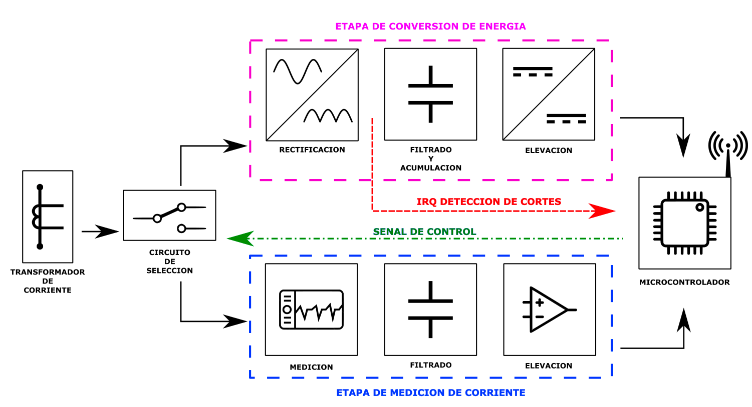
\includegraphics[width=.7\textwidth]{./Figuras/HW_block_diagram.png}
	\caption{Diagrama en bloques del hardware asociado al sistema.}
	\label{fig:diagBloques}
\end{figure}

\vspace{15px}
\begin{itemize}
	\item Transformador de Corriente (TI): encargado de suplir de corriente eléctrica para la carga del acumulador, como así también actuar como  transductor de corriente para la medición del valor eficaz de la misma.\\

	\item Etapa de conversión y acumulación de energía: compuesta por un rectificador de baja caída, un acumulador y un conversor DC/DC.\\

	\item Etapa de medición / detección de corriente: encargado de las mediciones de valor eficaz de corriente alterna junto a un circuito de acondicionamiento de señal.\\

	\item Circuito de selección de modo: compuesto por un relay (RL) acorde al TI y su circuito de excitación.\\

	\item Etapa de procesamiento, control y comunicaciones: compuesto por un microcontrolador (uC) y un módulo de comunicaciones (MC) LoRa.\\
\end{itemize}

\subsection{Servicios de Backend a desarrollar}
Para lograr la recuperación de datos generados por el HW y enviados a la red LoRaWAN, es necesario contar con un conjunto de servicios privados de backend (BES). Estos deberán estar integrados de manera permanente con la red LoRaWAN la cual se considera ya existente cuya infraestructura es presentada en la Figura \ref{fig:diagBloquesLoRaWAN}.\\

\begin{figure}[H]
	\centering 
	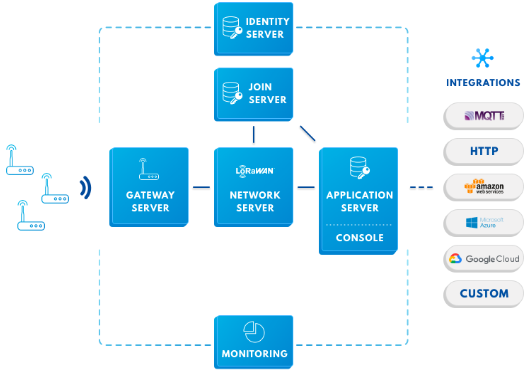
\includegraphics[width=.7\textwidth]{./Figuras/arquitectura_TTN.png}
	\caption{Diagrama en bloques de la red LoRaWAN a utilizar y sus posibles integraciones con terceras partes.}
	\label{fig:diagBloquesLoRaWAN}
\end{figure}

Esta integración se logrará a través de APIs HTTP o mediante suscripciones a tópicos de broker de mensajería.\\
Los BES privados a desarrollar en este proyecto serán 3:
\begin{enumerate}
	\item Servicio de Recuperación de Datos: encargado de recuperar los datos enviados por los nodos a traves de la API proporcionada por TTN y almacenarlos en una base de datos.
	\item Base de Datos (DB): encargado de almacenar los valores históricos de los nodos sensores y generar diferentes métricas para los reportes de estado para luego desplegarlas en una interfaz gráfica de usuario.
	\item Interfaz Gráfica de Usuario (GUI): encargada de presentar los últimos datos recuperados por cada nodo de manera amigable para el usuario final del sistema.
\end{enumerate}

\end{consigna}


\section{Identificación y análisis de los interesados}
\label{sec:interesados}

\begin{consigna}{black} 

\begin{table}[H]
%\caption{Identificación de los interesados}
%\label{tab:interesados}
\begin{tabularx}{\linewidth}{@{}|l|X|X|l|@{}}
\hline
\rowcolor[HTML]{C0C0C0} 
Rol           & Nombre y Apellido & Organización 	& Puesto 	\\ \hline
Auspiciante, Impulsor\\Responsable y Equipo  	    & Ing. Milton E. Sosa & Universidad Nacional de Misiones &Egresado   	\\ \hline
Orientador    & \supname	      & \pertesupname 	& Director	Trabajo final \\ \hline
Colaboradores & Dr. Ing. Eduardo O. Sosa                  &Universidad Nacional de Misiones             	&Docente Investigador    	\\ \hline

\end{tabularx}
\end{table}
 
\begin{itemize}
\item Ing. Marcelo E. Romeo, de vasta experiencia profesional en el ámbito de la microelectrónica e investigación y desarrollo para diferentes entidades y universidades nacionales.
\item Dr. Ing. Eduardo O. Sosa, cuenta con más de 20 años de experiencia en el área de las TELCO, ex miembro colaborador de la RIU, profesor titular de la cátedra de Física en la Universidad Nacional de Misiones y lidera proyectos bilaterales entre Argentina y Alemania en el ámbito de IoT.
\end{itemize}

\end{consigna}


\section{1. Propósito del proyecto}
\label{sec:proposito}

\begin{consigna}{black}
El propósito de este proyecto es el de desarrollar un sistema formado por un circuito electrónico autónomo y un conjunto de software dedicado a la recuperación y almacenamiento de datos generados y transmitidos por el circuito.\\
El mismo, debe ser capaz de permitir a las actuales redes de distribución de energía eléctrica reportar su estado actual de operación al centro de monitoreo.
\end{consigna}

\section{2. Alcance del proyecto}
\label{sec:alcance}

\begin{consigna}{black}
Se pretende desarrollar un prototipo de HW capaz de ser autosuficiente en cuanto a la conversión, acumulación y gestión de energía eléctrica con el objeto de alimentar y permitir su operación en estado autónomo y permanente. Para ello se desarrollará un circuito de micro energy harvesting basado en rectificadores de bajas pérdidas, acumuladores aptos para la aplicación final y un conversor DC/DC de alta eficiencia.\\
Se desarrollará una etapa de medición de valor eficaz de corriente alterna, con el objeto de medir la intensidad de corriente que actualmente circula por el conductor conectado a la salida de baja tensión e inmediatamente después del fusible aéreo de protección.\\
Agregado a los módulos mencionados anteriormente, un microcontrolador se encargará de la gestión de energía de todo el HW y de digitalizar todas las mediciones realizadas para finalmente enviarlas al centro de operaciones a traves de un módulo de comunicación.\\
Los BES se albergaran en una computadora de bajo costo la cual proporcionará suficientes recursos para su operación y ensayo en la etapa de desarollo.\\

No es parte del alcance del presente proyecto llegar a una etapa de lanzamiento del producto a clientes finales, sino la de lograr un demostrador tecnológico. Sin embargo, si los tiempos lo permiten y se logra contar con una infraestructura adecuada, se desean realizar ensayos end-to-end en laboratorio sobre el sistema, involucrando los prototipos de hardware que fueran desarrollados, y una integración mínima entre los BES y la red LoRaWAN ya existente.\\
\end{consigna}


\section{3. Supuestos del proyecto}
\label{sec:supuestos}
\begin{consigna}{black}
Para el desarrollo del presente proyecto se supone que:
\begin{itemize}
\item El autor del trabajo no tendrá ningún problema para hacerse de los insumos necesarios para alcanzar los objetivos incurriendo a distribuidores de componentes en el mercado local.
\item Al momento de ensayar el sistema, se debe contar con acceso a una red LoRaWAN operativa como por ejemplo The Things Network.
\item El autor no tendrá en ningún momento limitaciones de movilidad.
\item En caso de ser necesario realizar ensayos end-to-end, el autor deberá incurrir en la fabricación de un banco de ensayos apropiado para simular los casos de uso y probar el sistema en su conjunto como así disponer de instrumentos patrones para contrastar y verificar el correcto funcionamiento, pudiendo así impactar la fecha final de entrega de los items listados en el punto 5.
\end{itemize}

\end{consigna}

\section{4. Requerimientos}
\label{sec:requerimientos}
\begin{consigna}{black}
\begin{enumerate}
\item Grupo de requerimientos asociados con hardware
	\begin{enumerate}
	\item Respetuoso con el medioambiente.
	\item Compacto.
	\item De fácil comisionamiento y puesta en funcionamiento.
	\item Bajo consumo en modo ocioso.
	\item Mínimo mantenimiento in-situ.
	\item Agnóstico a la frecuencia de operación de la red 50/60 Hz.
	\item Agnóstico a la tensión de fase del sistema de distribución 110/220 Voltios.
	\end{enumerate}
\item Grupo de requerimientos asociados con software
	\begin{enumerate}
	\item Tanto el software a desarrollar para el firmware del microcontrolador, como para los BES se deberán desarrollar haciendo uso de un lenguaje que permita celeridad en el desarrollo, fácil integración entre ambas partes, ensayos, verificaciones y futuro mantenimiento.
	\end{enumerate}
\item Grupo de requerimientos asociados con ensayos de integración
\begin{enumerate}
	\item Red LoRaWAN disponible y operativa con buena cobertura.
	\item Conectividad a internet para verificación de correcto funcionamiento del sistema.
\end{enumerate}
\end{enumerate}


\end{consigna}

\section{5. Entregables principales del proyecto}
\label{sec:entregables}

\begin{consigna}{black}
\begin{itemize}
\item Diagrama esquemático
\item Código fuente del firmware 
\item Diagrama de instalación
\item Informe final

\end{itemize}

\end{consigna}

\section{6. Desglose del trabajo en tareas}
\label{sec:wbs}
\begin{consigna}{black}
\begin{enumerate}
\item Grupo de tareas asociadas al hardware (Total: 472 hs)
	\begin{enumerate}
			 \item Transductor de corriente. (Total: 20 hs)
			 \begin{enumerate}
			 	\item Análisis de transductores aptos para el hardware a desarrollar. (5 hs)
			 	\item Selección de componentes. (5 hs)
			 	\item Ensayo y evaluación del transductor de manera individual. (10 hs)
			 \end{enumerate}
			
			 \item Etapa de circuito de selección. (Total: 20 hs)
			 \begin{enumerate}
			 	\item Análisis de alternativas técnicas. (10 hs)
			 	\item Selección de componentes en base a los requerimientos de hardware presentados en el punto \ref{sec:requerimientos}. (6 hs)
			 	\item Ensayo del circuito de selección de manera individual. (4 hs)
			 \end{enumerate}			
			
			 \item Etapa de rectificación y filtrado. (Total: 53 hs)
			 \begin{enumerate}
				\item Análisis comparativo de alternativas para técnicas de rectificacion. (30 hs)
				\item Selección de componentes encargados de la etapa de rectificación. (10 hs)
				\item Ensayo de la etapa de rectificación de manera individual. (5 hs)
				\item Evaluación de resultados. (8 hs)
			 \end{enumerate}
			
			 \item Etapa de acumulación de energía. (Total: 60 hs)
			 \begin{enumerate}
			 	\item Análisis de alternativas viables para acumulación de energía acorde a los requerimientos de hardware presentados en la etapa \ref{sec:requerimientos}. (10 hs)
			 	\item Selección de la etapa de acumulacion de energía. (15 hs)
			 	\item Ensayo de la etapa de acumulación de energía de manera individual. (20 hs)
			 	\item Evaluación de resultados y estimación de la autonomía de operación en función de diferentes perfiles de consumo. (15 hs)
			 \end{enumerate}
			 
			 \item Etapa de elevación de tensión. (Total: 20 hs)
			 \begin{enumerate}
			 	\item Análisis de alternativas técnicas para elevación de tensión aptas para el hardware a desarrollar. (15 hs)
			 	\item Ensayo y evaluación de la etapa de elevación de tensión de manera individual. (5 hs)
			 \end{enumerate}

			 \item Etapa de medición de corriente. (Total: 45 hs)
			 \begin{enumerate}
			 	\item Análisis de alternativas para realizar la medición del valor eficaz de corriente para el hardware a desarrollar. (20 hs)
			 	\item Selección de alternativa acorde a los requerimientos de hardware presentados en la etapa \ref{sec:requerimientos}. (15 hs)
			 	\item Ensayo y evaluación de la etapa de medición de valor eficaz de manera individual. (10 hs)
			 \end{enumerate}
			 
			 \item Etapa de elevación de tensión. (Total: 24 hs)
			 \begin{enumerate}
			 	\item Análisis de alternativas técnicas para filtrado y amplificación. (10 hs)
			 	\item Selección de componentes. (4 hs)
			 	\item Ensayo y evaluación de la etapa de filtrado y amplificación de manera individual. (10 hs)
			 \end{enumerate}
			 
			 \item Microcontrolador y módulo de comunicaciones-. (Total: 100 hs)
			 \begin{enumerate}
			 	\item Análisis de microcontroladores y módulos de comunicación aptos para la aplicación. (40 hs)
			 	\item Selección acorde al propósito y alcance del proyecto. (20 hs)
			 	\item Pruebas de laboratorio del microcontrolador y modulo de comunicación de manera individual. (40 hs)
			 \end{enumerate}
			 \item Circuito impreso. (Total: 130)
			 \begin{enumerate}
			 	\item Ruteo del circuito impreso. (60 hs)
			 	\item Inspección. (20 hs)
			 	\item Montaje y soldado de componentes. (40 hs)
			 	\item Depuración. (10 hs)
			 \end{enumerate}			 			 			 
		\end{enumerate}
				
	\item Grupo de tareas asociadas al software (Total: 220)
	\begin{enumerate}
		\item Tareas asociadas al firmware del microcontrolador (Total: 110 hs)
			\begin{enumerate}
				\item Definición de la "lógica de negocio" que regirá la operación del hardware a instalar in-situ. (10 hs)
				\item Prototipado del firmware. (60 hs)
				\item Depuración de errores. (20 hs)
				\item Pruebas unitarias. (20 hs)
			\end{enumerate}
		
		 \item Tareas asociadas a los BES (Total: 110 hs)
			\begin{enumerate}
				\item Definición de la lógica de operación de cada servicio. (20 hs)
				\item Desarrollo del software. (50 hs)
				\item Pruebas de integración. (20 hs)
				\item Depuración de errores. (20 hs)
			\end{enumerate}				
		
		\end{enumerate}
		
		 \item Tareas asociadas a pruebas de integración. (Total: 105 hs)
		 \begin{enumerate}
		 	\item Definición de los casos de ensayo. (20 hs)
		 	\item Desarrollo del software. (50 hs)
		 	\item Ejecución de las pruebas. (15 hs)
		 	\item Depuración de errores. (20 hs)
		 \end{enumerate}		
	\end{enumerate}

Cantidad total de horas: (797 hs)

\end{consigna}

\section{7. Diagrama de Activity On Node}
\label{sec:AoN}

\begin{consigna}{red}
Armar el AoN a partir del WBS definido en la etapa anterior. 

%La figura \ref{fig:AoN} fue elaborada con el paquete latex tikz y pueden consultar la siguiente referencia \textit{online}:

%\url{https://www.overleaf.com/learn/latex/LaTeX_Graphics_using_TikZ:_A_Tutorial_for_Beginners_(Part_3)\%E2\%80\%94Creating_Flowcharts}

\end{consigna}

\begin{figure}[htpb]
\centering 
\includegraphics[width=.8\textwidth]{./Figuras/AoN.png}
\caption{Diagrama en \textit{Activity on Node}}
\label{fig:AoN}
\end{figure}

Indicar claramente en qué unidades están expresados los tiempos.
De ser necesario indicar los caminos semicríticos y analizar sus tiempos mediante un cuadro.
Es recomendable usar colores y un cuadro indicativo describiendo qué representa cada color, como se muestra en el siguiente ejemplo:



\section{8. Diagrama de Gantt}
\label{sec:gantt}

\begin{consigna}{red}
Utilizar el software Gantter for Google Drive o alguno similar para dibujar el diagrama de Gantt.

Existen muchos programas y recursos \textit{online} para hacer diagramas de gantt, entre las cuales destacamos:

\begin{itemize}
\item Planner
\item GanttProject
\item Trello + \textit{plugins}. En el siguiente link hay un tutorial oficial: \\ \url{https://blog.trello.com/es/diagrama-de-gantt-de-un-proyecto}
\item Creately, herramienta online colaborativa. \\\url{https://creately.com/diagram/example/ieb3p3ml/LaTeX}
\item Se puede hacer en latex con el paquete \textit{pgfgantt}\\ \url{http://ctan.dcc.uchile.cl/graphics/pgf/contrib/pgfgantt/pgfgantt.pdf}
\end{itemize}

Pegar acá una captura de pantalla del diagrama de Gantt, cuidando que la letra sea suficientemente grande como para ser legible. 
Si el diagrama queda demasiado ancho, se puede pegar primero la ``tabla'' del Gantt y luego pegar la parte del diagrama de barras del diagrama de Gantt.

Configurar el software para que en la parte de la tabla muestre los códigos del EDT (WBS).\\
Configurar el software para que al lado de cada barra muestre el nombre de cada tarea.\\
Revisar que la fecha de finalización coincida con lo indicado en el Acta Constitutiva.

En la figura \ref{fig:gantt}, se muestra un ejemplo de diagrama de gantt realizado con el paquete de \textit{pgfgantt}. En la plantilla pueden ver el código que lo genera y usarlo de base para construir el propio.

\begin{figure}[htbp]
\begin{center}
\begin{ganttchart}{1}{12}
  \gantttitle{2020}{12} \\
  \gantttitlelist{1,...,12}{1} \\
  \ganttgroup{Group 1}{1}{7} \\
  \ganttbar{Task 1}{1}{2} \\
  \ganttlinkedbar{Task 2}{3}{7} \ganttnewline
  \ganttmilestone{Milestone o hito}{7} \ganttnewline
  \ganttbar{Final Task}{8}{12}
  \ganttlink{elem2}{elem3}
  \ganttlink{elem3}{elem4}
\end{ganttchart}
\end{center}
\caption{Diagrama de gantt de ejemplo}
\label{fig:gantt}
\end{figure}

\end{consigna}

\section{9. Matriz de uso de recursos de materiales}
\label{sec:recursos}


\begin{table}[htpb]
\label{tab:recursos}
\centering
\begin{tabularx}{\linewidth}{@{}|c|X|X|X|X|X|@{}}
\hline
\cellcolor[HTML]{C0C0C0} & \cellcolor[HTML]{C0C0C0} & \multicolumn{4}{c|}{\cellcolor[HTML]{C0C0C0}Recursos requeridos (horas)} \\ \cline{3-6} 
\multirow{-2}{*}{\cellcolor[HTML]{C0C0C0}\begin{tabular}[c]{@{}c@{}}Código\\ WBS\end{tabular}} & \multirow{-2}{*}{\cellcolor[HTML]{C0C0C0}\begin{tabular}[c]{@{}c@{}}Nombre \\ tarea\end{tabular}} & Material 1 & Material 2 & Material 3 & Material 4 \\ \hline
 &  &  &  &  &  \\ \hline
 &  &  &  &  &  \\ \hline
 &  &  &  &  &  \\ \hline
 &  &  &  &  &  \\ \hline
\end{tabularx}%
\end{table}


\section{10. Presupuesto detallado del proyecto}
\label{sec:presupuesto}

\begin{consigna}{red}
Si el proyecto es complejo entonces separarlo en partes:
\begin{itemize}
\item Un total global, indicando el subtotal acumulado por cada una de las áreas.
\item El desglose detallado del subtotal de cada una de las áreas.
\end{itemize}

IMPORTANTE: No olvidarse de considerar los COSTOS INDIRECTOS.

\end{consigna}

\begin{table}[htpb]
\centering
\begin{tabularx}{\linewidth}{@{}|X|c|r|r|@{}}
\hline
\rowcolor[HTML]{C0C0C0} 
\multicolumn{4}{|c|}{\cellcolor[HTML]{C0C0C0}COSTOS DIRECTOS} \\ \hline
\rowcolor[HTML]{C0C0C0} 
Descripción &
  \multicolumn{1}{c|}{\cellcolor[HTML]{C0C0C0}Cantidad} &
  \multicolumn{1}{c|}{\cellcolor[HTML]{C0C0C0}Valor unitario} &
  \multicolumn{1}{c|}{\cellcolor[HTML]{C0C0C0}Valor total} \\ \hline
 &
  \multicolumn{1}{c|}{} &
  \multicolumn{1}{c|}{} &
  \multicolumn{1}{c|}{} \\ \hline
 &
  \multicolumn{1}{c|}{} &
  \multicolumn{1}{c|}{} &
  \multicolumn{1}{c|}{} \\ \hline
\multicolumn{1}{|l|}{} &
   &
   &
   \\ \hline
\multicolumn{1}{|l|}{} &
   &
   &
   \\ \hline
\multicolumn{3}{|c|}{SUBTOTAL} &
  \multicolumn{1}{c|}{} \\ \hline
\rowcolor[HTML]{C0C0C0} 
\multicolumn{4}{|c|}{\cellcolor[HTML]{C0C0C0}COSTOS INDIRECTOS} \\ \hline
\rowcolor[HTML]{C0C0C0} 
Descripción &
  \multicolumn{1}{c|}{\cellcolor[HTML]{C0C0C0}Cantidad} &
  \multicolumn{1}{c|}{\cellcolor[HTML]{C0C0C0}Valor unitario} &
  \multicolumn{1}{c|}{\cellcolor[HTML]{C0C0C0}Valor total} \\ \hline
\multicolumn{1}{|l|}{} &
   &
   &
   \\ \hline
\multicolumn{1}{|l|}{} &
   &
   &
   \\ \hline
\multicolumn{1}{|l|}{} &
   &
   &
   \\ \hline
\multicolumn{3}{|c|}{SUBTOTAL} &
  \multicolumn{1}{c|}{} \\ \hline
\rowcolor[HTML]{C0C0C0}
\multicolumn{3}{|c|}{TOTAL} &
   \\ \hline
\end{tabularx}%
\end{table}


\section{11. Matriz de asignación de responsabilidades}
\label{sec:responsabilidades}
\begin{consigna}{red}
Establecer la matriz de asignación de responsabilidades y el manejo de la autoridad completando la siguiente tabla:

\begin{table}[htpb]
\centering
\resizebox{\textwidth}{!}{%
\begin{tabular}{|c|c|c|c|c|c|}
\hline
\rowcolor[HTML]{C0C0C0} 
\cellcolor[HTML]{C0C0C0} &
  \cellcolor[HTML]{C0C0C0} &
  \multicolumn{4}{c|}{\cellcolor[HTML]{C0C0C0}Listar todos los nombres y roles del proyecto} \\ \cline{3-6} 
\rowcolor[HTML]{C0C0C0} 
\cellcolor[HTML]{C0C0C0} &
  \cellcolor[HTML]{C0C0C0} &
  Responsable &
  Orientador &
  Equipo &
  Cliente \\ \cline{3-6} 
\rowcolor[HTML]{C0C0C0} 
\multirow{-3}{*}{\cellcolor[HTML]{C0C0C0}\begin{tabular}[c]{@{}c@{}}Código\\ WBS\end{tabular}} &
  \multirow{-3}{*}{\cellcolor[HTML]{C0C0C0}Nombre de la tarea} &
  \authorname &
  \supname &
  Nombre de alguien &
  \clientename \\ \hline
 &  &  &  &  &  \\ \hline
 &  &  &  &  &  \\ \hline
 &  &  &  &  &  \\ \hline
\end{tabular}%
}
\end{table}

{\footnotesize
Referencias:
\begin{itemize}
	\item P = Responsabilidad Primaria
	\item S = Responsabilidad Secundaria
	\item A = Aprobación
	\item I = Informado
	\item C = Consultado
\end{itemize}
} %footnotesize

Una de las columnas debe ser para el Director, ya que se supone que participará en el proyecto.
A su vez se debe cuidar que no queden muchas tareas seguidas sin ``A'' o ``I''.

Importante: es redundante poner ``I/A'' o ``I/C'', porque para aprobarlo o responder consultas primero la persona debe ser informada.

\end{consigna}

\section{12. Gestión de riesgos}
\label{sec:riesgos}

\begin{consigna}{red}
a) Identificación de los riesgos (al menos cinco) y estimación de sus consecuencias:
 
Riesgo 1: detallar el riesgo (riesgo es algo que si ocurre altera los planes previstos)
\begin{itemize}
\item Severidad (S): mientras más severo, más alto es el número (usar números del 1 al 10).\\
Justificar el motivo por el cual se asigna determinado número de severidad (S).
\item Probabilidad de ocurrencia (O): mientras más probable, más alto es el número (usar del 1 al 10).\\
Justificar el motivo por el cual se asigna determinado número de (O). 
\end{itemize}   

Riesgo 2:
\begin{itemize}
\item Severidad (S): 
\item Ocurrencia (O):
\end{itemize}

Riesgo 3:
\begin{itemize}
\item Severidad (S): 
\item Ocurrencia (O):
\end{itemize}


b) Tabla de gestión de riesgos:      (El RPN se calcula como RPN=SxO)

\begin{table}[htpb]
\centering
\begin{tabularx}{\linewidth}{@{}|X|c|c|c|c|c|c|@{}}
\hline
\rowcolor[HTML]{C0C0C0} 
Riesgo & S & O & RPN & S* & O* & RPN* \\ \hline
       &   &   &     &    &    &      \\ \hline
       &   &   &     &    &    &      \\ \hline
       &   &   &     &    &    &      \\ \hline
       &   &   &     &    &    &      \\ \hline
       &   &   &     &    &    &      \\ \hline
\end{tabularx}%
\end{table}

Criterio adoptado: 
Se tomarán medidas de mitigación en los riesgos cuyos números de RPN sean mayores a ....

Nota: los valores marcados con (*) en la tabla corresponden luego de haber aplicado la mitigación.

c) Plan de mitigación de los riesgos que originalmente excedían el RPN máximo establecido:
 
Riesgo 1: Plan de mitigación (si por el RPN fuera necesario elaborar un plan de mitigación).
  Nueva asignación de S y O, con su respectiva justificación:
  - Severidad (S): mientras más severo, más alto es el número (usar números del 1 al 10).
          Justificar el motivo por el cual se asigna determinado número de severidad (S).
  - Probabilidad de ocurrencia (O): mientras más probable, más alto es el número (usar del 1 al 10).
          Justificar el motivo por el cual se asigna determinado número de (O).

Riesgo 2: Plan de mitigación (si por el RPN fuera necesario elaborar un plan de mitigación).
 
Riesgo 3: Plan de mitigación (si por el RPN fuera necesario elaborar un plan de mitigación)

\end{consigna}


\section{13. Gestión de la calidad}
\label{sec:calidad}

\begin{consigna}{red}
Para cada uno de los requerimientos del proyecto indique:
\begin{itemize} 
\item Req \#1: Copiar acá el requerimiento.

Verificación y validación:

\begin{itemize}
\item Verificación para confirmar si se cumplió con lo requerido antes de mostrar el sistema al cliente:\\
Detallar 
\item Validación con el cliente para confirmar que está de acuerdo en que se cumplió con lo requerido:\\
Detallar  
\end{itemize}

\end{itemize}

Tener en cuenta que en este contexto se pueden mencionar simulaciones, cálculos, revisión de hojas de datos, consulta con expertos, etc.

\end{consigna}

\section{14. Comunicación del proyecto}
\label{sec:comunicaciones}

\begin{consigna}{red}
El plan de comunicación del proyecto es el siguiente:
\end{consigna}

% Please add the following required packages to your document preamble:
% \usepackage{graphicx}
% \usepackage[table,xcdraw]{xcolor}
% If you use beamer only pass "xcolor=table" option, i.e. \documentclass[xcolor=table]{beamer}
\begin{table}[htpb]
\centering
\resizebox{\textwidth}{!}{%
\begin{tabular}{|c|c|c|c|c|c|}
\hline
\rowcolor[HTML]{C0C0C0} 
\multicolumn{6}{|c|}{\cellcolor[HTML]{C0C0C0}PLAN DE COMUNICACIÓN DEL PROYECTO}           \\ \hline
\rowcolor[HTML]{C0C0C0} 
¿Qué comunicar? & Audiencia & Propósito & Frecuencia & Método de comunicac. & Responsable \\ \hline
                &           &           &            &                      &             \\ \hline
                &           &           &            &                      &             \\ \hline
                &           &           &            &                      &             \\ \hline
                &           &           &            &                      &             \\ \hline
                &           &           &            &                      &             \\ \hline
\end{tabular}%
}
\end{table}

\section{15. Gestión de Compras}
\label{sec:compras}

\begin{consigna}{red}
En caso de tener que comprar elementos o contratar servicios:
a) Explique con qué criterios elegiría a un proveedor.
b) Redacte el Statement of Work correspondiente.
\end{consigna}

\section{16. Seguimiento y control}
\label{sec:seguimiento}

\begin{consigna}{red}
Para cada tarea del proyecto establecer la frecuencia y los indicadores con los se seguirá su avance y quién será el responsable de hacer dicho seguimiento y a quién debe comunicarse la situación (en concordancia con el Plan de Comunicación del proyecto).

El indicador de avance tiene que ser algo medible, mejor incluso si se puede medir en \% de avance. Por ejemplo,se pueden indicar en esta columna cosas como ``cantidad de conexiones ruteadeas'' o ``cantidad de funciones implementadas'', pero no algo genérico y ambiguo como ``\%'', porque el lector no sabe porcentaje de qué cosa.

\end{consigna}

\begin{table}[!htpb]
\centering
\begin{tabularx}{\linewidth}{@{}|X|X|X|X|X|X|@{}}
\hline
\rowcolor[HTML]{C0C0C0} 
\multicolumn{6}{|c|}{\cellcolor[HTML]{C0C0C0}SEGUIMIENTO DE AVANCE}                                                                       \\ \hline
\rowcolor[HTML]{C0C0C0} 
Tarea del WBS & Indicador de avance & Frecuencia de reporte & Resp. de seguimiento & Persona a ser informada & Método de comunic. \\ \hline
 &  &  &  &  &  \\ \hline
 &  &  &  &  &  \\ \hline
 &  &  &  &  &  \\ \hline
 &  &  &  &  &  \\ \hline
 &  &  &  &  &  \\ \hline
\end{tabularx}%
%}
\end{table}

\section{17. Procesos de cierre}    
\label{sec:cierre}

\begin{consigna}{red}
Establecer las pautas de trabajo para realizar una reunión final de evaluación del proyecto, tal que contemple las siguientes actividades:

\begin{itemize}
\item Pautas de trabajo que se seguirán para analizar si se respetó el Plan de Proyecto original:
 - Indicar quién se ocupará de hacer esto y cuál será el procedimiento a aplicar. 
\item Identificación de las técnicas y procedimientos útiles e inútiles que se utilizaron, y los problemas que surgieron y cómo se solucionaron:
 - Indicar quién se ocupará de hacer esto y cuál será el procedimiento para dejar registro.
\item Indicar quién organizará el acto de agradecimiento a todos los interesados, y en especial al equipo de trabajo y colaboradores:
  - Indicar esto y quién financiará los gastos correspondientes.
\end{itemize}

\end{consigna}


\end{document}
